\chapter{Convolutional Neural Networks (CNNs)}
\label{ch:lesson34}

The layers in Chapters~\ref{ch:lesson31}--\ref{ch:lesson33} treat every input as a flat vector, and that creates two distinct problems for images. First, each pixel gets its own independent weight, with no notion that neighboring pixels are \emph{near} each other --- the entire spatial structure images have is thrown away. Second, because every position gets its own separate weights, a fully-connected layer has no way to reuse a filter it's already learned: it must independently re-learn what an edge looks like at every single position, all over again. \textbf{Convolution} --- already built manually in Chapter~\ref{ch:lesson10} --- fixes both problems at once by baking in an \textbf{inductive bias}: restrict each output to a small local patch, and share that patch's weights across every position.

\section{A conv layer is a projection, restricted and shared}

Recall Chapter~\ref{ch:lesson30}'s central idea: $y=w^\top x+b$, a projection. A convolutional layer computes \emph{exactly this}, but for $x$, it only looks at a small local patch (say $3\times3$) instead of the whole image --- and, crucially, it reuses the \emph{same} $w$ at every patch location. Two consequences:
\begin{itemize}
  \item \textbf{Vastly fewer parameters.} A $3\times3$ filter over a single input channel has 9 weights, no matter how big the image is --- a fully-connected layer over a $16\times16$ image needs 256 weights \emph{per output unit}.
  \item \textbf{Translation equivariance.} Because the same filter slides everywhere, a feature learned at one position is automatically detected at every other position too, for free. \emph{Equivariant} means the output shifts along with the input, rather than staying fixed --- shift the image by 2 pixels and the feature map's detections shift by exactly 2 pixels too. That's a distinct, weaker property than \emph{invariance} (an unchanged output despite a shifted input), which pooling adds a bit of, later in this chapter.
\end{itemize}

\subsection*{A conv layer kernel is 3D}

A ``$3\times3$ filter'' in a CNN is really $3\times3\times C_{in}$, not just $3\times3$. Chapter~\ref{ch:lesson10}'s kernels were flat 2D grids, because they slid over a single grayscale channel. A conv layer's filter has to reach across \emph{every} input channel at once --- a $3\times3$ filter on a 3-channel RGB image has $3\times3\times3=27$ weights, one full depth-slice per input channel, summed together into a single output value at each position. Stack $C_{out}$ of these $3\times3\times C_{in}$ filters side by side (one per output channel) and the full weight tensor is 4D: \code{(C\_out, C\_in, 3, 3)}.

\section{Conv2d, forward and backward, from scratch}

This is the same sliding-window computation as Chapter~\ref{ch:lesson10}'s convolution, just with the kernel now a set of \emph{learnable} weights instead of a fixed, hand-designed one --- which means it needs a backward pass too.

\begin{lstlisting}
def conv2d_forward(img, kernel, bias):
    N, C, H, W = img.shape
    OC, IC, KH, KW = kernel.shape
    OH, OW = H - KH + 1, W - KW + 1
    out = np.zeros((N, OC, OH, OW))
    for n in range(N):
        for oc in range(OC):
            for i in range(OH):
                for j in range(OW):
                    patch = img[n, :, i:i+KH, j:j+KW]
                    out[n, oc, i, j] = np.sum(patch * kernel[oc]) + bias[oc]
    return out
\end{lstlisting}

A from-scratch forward pass matches \code{F.conv2d} to $8.88\times10^{-16}$; the from-scratch backward pass matches PyTorch autograd's gradients on the input, kernel, and bias to $8.88\times10^{-16}$, $7.99\times10^{-15}$, and $1.78\times10^{-15}$ respectively.

\subsection*{Filters you already know: Chapter~\ref{ch:lesson12}'s edge detectors}

The output of a conv layer before training is nonsense; the point is that gradient descent will \emph{find} useful filters. To see what a useful filter's output already looks like, apply a filter designed by hand back in Chapter~\ref{ch:lesson12}: Sobel's edge kernel. As it turns out, trained CNNs' first-layer filters often converge to something visually similar to this --- oriented edge and blob detectors --- regardless of what the network was trained to do (Figure~\ref{fig:l34-1}).

\begin{figure}[h]
\centering
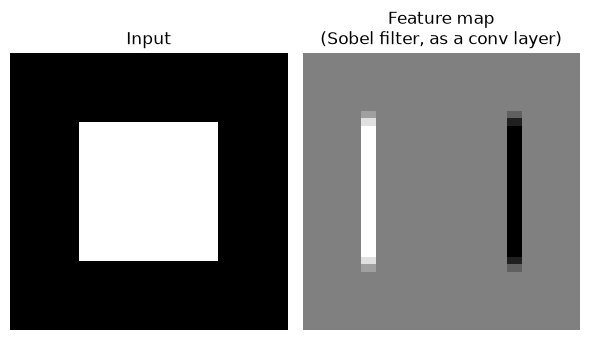
\includegraphics[width=0.5\textwidth]{figures/lesson34_fig01.png}
\caption{Sobel's edge kernel, applied as a conv layer, on a simple square.}
\label{fig:l34-1}
\end{figure}

\section{Pooling: downsampling with a purpose}

\textbf{Max pooling} slides a window over the feature map and keeps only the maximum value in each window, shrinking the spatial size (like the pyramids of Chapter~\ref{ch:lesson11}) while adding a small amount of local translation invariance --- a feature detected at slightly different positions within one pooling window still produces the same output. A from-scratch $2\times2$ max pool matches \code{F.max\_pool2d} exactly (max diff $0.00\times10^{0}$).

\section{Putting them together: convolution and pooling, interleaved}

A real CNN is neither all convolution nor all pooling --- it's the two stacked in alternation: convolution, pooling, convolution, pooling, and so on. Each pooling step roughly \emph{halves} the spatial size ($H$ and $W$), and the rule of thumb is to roughly \emph{double} the number of channels in the conv layer that follows. That's not a coincidence: pooling throws away spatial resolution, so doubling the channel count right after keeps the total amount of information ($C\times H\times W$) roughly constant from stage to stage, even as the representation trades ``a little detail at many positions'' for ``more detail at fewer positions.''

\section{Why translation equivariance actually matters: a generalization test}

Build a small classification task: a $16\times16$ image contains either a plus sign or a circle, at a \emph{random position}. Train on shapes placed only near the center; test on shapes placed only near the corners --- positions the model never saw during training (Figure~\ref{fig:l34-2}). A network that has genuinely learned ``what a plus looks like,'' rather than ``which pixels tend to be on for a plus at these particular training positions,'' should have no trouble with this.

\begin{figure}[h]
\centering
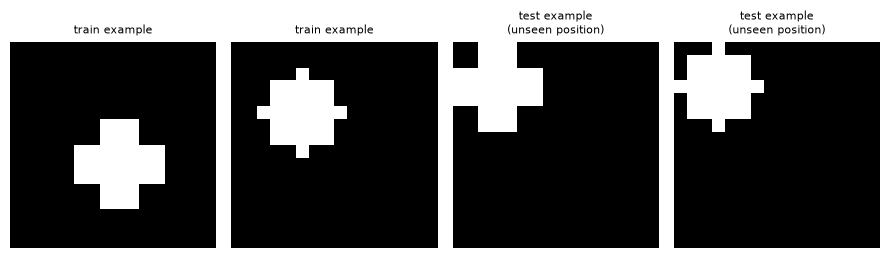
\includegraphics[width=0.9\textwidth]{figures/lesson34_fig02.png}
\caption{Train examples (centered positions) vs.\ test examples (unseen, corner positions).}
\label{fig:l34-2}
\end{figure}

\begin{lstlisting}
class CNNClassifier(nn.Module):
    def __init__(self):
        super().__init__()
        self.conv = nn.Sequential(
            nn.Conv2d(1, 8, 5, padding=2), nn.ReLU(),
            nn.MaxPool2d(2),
            nn.Conv2d(8, 16, 5, padding=2), nn.ReLU(),
            nn.AdaptiveMaxPool2d(1),  # global max pool: collapses ALL spatial position info
        )
        self.fc = nn.Linear(16, 1)
\end{lstlisting}

Training a flatten-based MLP and this CNN on the same data:

\begin{center}
\renewcommand{\arraystretch}{1.3}
\begin{tabular}{lrr}
\hline
\textbf{model} & \textbf{train acc} & \textbf{test acc (unseen positions)} \\
\hline
MLP & 100.0\% & 73.3\% \\
CNN & 100.0\% & 100.0\% \\
\hline
\end{tabular}
\end{center}

Both models fit the training data perfectly. On positions neither has ever seen, the flatten-based MLP does little better than a coin flip --- it memorized \emph{which pixels} tend to be on for each class at the training positions, and that knowledge doesn't transfer. The CNN, whose global max pooling forces the final decision to depend only on \emph{what filters fired somewhere}, not \emph{where}, generalizes to the new positions with no loss in accuracy at all.

\subsection*{Exercises}
\begin{enumerate}
  \item Replace \code{nn.AdaptiveMaxPool2d(1)} in \code{CNNClassifier} with \code{nn.Flatten()} directly on the conv features (removing the global pooling, so spatial position is preserved all the way to the final linear layer). Retrain and re-evaluate on the unseen-position test set. Does the CNN's generalization advantage survive?
  \item Increase the gap between train and test position ranges, right at the image border where shapes get clipped. Does the CNN's accuracy hold up, or does it degrade --- and if it degrades, is that a translation-invariance failure or something else entirely (think about what happens to a shape's \emph{appearance}, not just its position, right at an edge)?
  \item \code{conv2d\_forward} above pads nothing, so the output shrinks with every layer. Modify it to support zero-padding and confirm the output size matches the input size, validated against \code{F.conv2d(..., padding=1)}.
\end{enumerate}

\vfill
\fullcode{lesson34}{lesson34_convolutional_neural_networks}
